\chapter{Introduction}
\label{cha:intro}

\section{Project Context and Motivation}
\label{sec:context}

The \ac{CSD3} is an \ac{EPSRC} Tier-2 national \ac{HPC} service hosted by the University of Cambridge \ac{RCS}, supporting computationally intensive research across a wide range of scientific disciplines \citep{ResearchComputingServicesDocumentation}. Effective use of such systems requires users to be able to follow and understand detailed documentation. These resources are often scattered across multiple sources, ranging from local \ac{CSD3} documentation \citep{ResearchComputingServicesDocumentation} to external resources such as package documentation, creating a barrier for new users \citep{AskHPC}.

As a result of this complexity, users frequently turn to the \ac{RCS} helpdesk for support. Figure \ref{fig:ticket-counts} shows that there has been a steady increase in the yearly number of resolved \ac{CSD3} helpdesk tickets from 2017 to 2025. This growth indicates not only sustained support demand, but also an expanding archive of operational support knowledge that could be reused to improve user support \citep{joslinGeneratingFrequentlyAsked2025}.

\begin{figure}[ht]
    \centering
    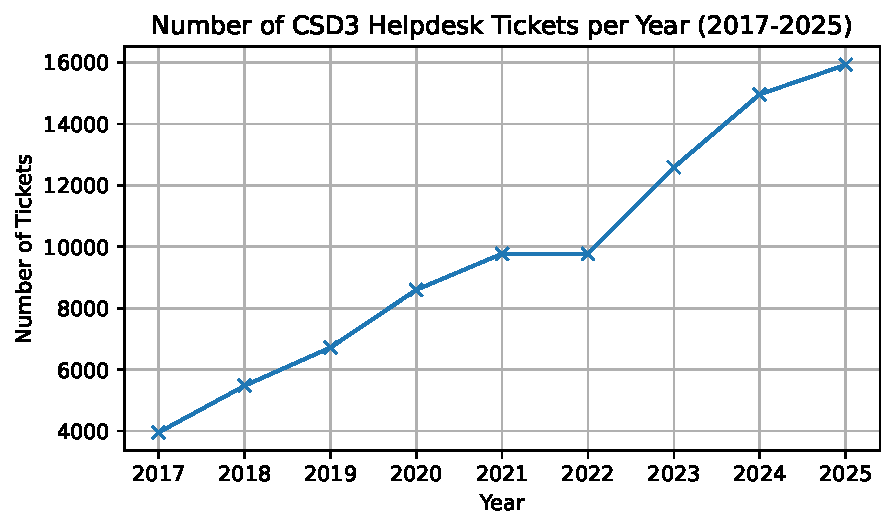
\includegraphics{graphs/ticket_counts.pdf}
    \caption{Annual number of resolved \acs{CSD3} helpdesk tickets from 2017 to 2025. Data sourced from \acs{RCS} support ticket records.}
    \label{fig:ticket-counts}
\end{figure}

Recent work has shown that \ac{RAG} is a promising approach for technical support \ac{QA} because it combines language generation with access to external evidence \citep{AskHPC,lewisRetrievalaugmentedGenerationKnowledgeintensive2020}. However, in heterogeneous support environments, answer quality depends not only on topical relevance, but also on whether the retrieved evidence is authoritative, current, and applicable to the local system state \citep{liYouKnowWhat2024,hwangRetrievalAugmentedGenerationEstimation2025}. In the \ac{CSD3} setting, this matters because local documentation, external package documentation, and historical support tickets play different evidential roles. The central challenge is therefore to retrieve evidence that is not just similar to the query, but suitable for the current \ac{CSD3} context. 

\section{Problem Definition and Scope}
\label{sec:problem}

This dissertation studies evidence-grounded first-response assistance for \ac{CSD3} support queries within a supervised internal workflow. The system is limited to single-hop questions, that is, queries answerable in one retrieval step from text-accessible evidence drawn from local documentation, selected external documentation, and visible ticket content. It does not attempt autonomous resolution and excludes attachment-dependent or multimodal evidence such as screenshots and log files. These boundaries keep the task operationally realistic while allowing later experiments to isolate the effect of heterogeneous-source retrieval and validity-aware reranking. 

\section{Research Questions and Hypotheses}
\label{sec:questions}

To investigate the problems introduced by the heterogeneous evidence base, this project addresses the following research questions (RQ), along with the associated hypotheses (H):

\begin{itemize}
    \item \textbf{RQ1:} \label{rq:1-source} Does combining local \ac{CSD3} documentation with historical support-ticket evidence improve the factual correctness of answers, relative to single-source retrieval?
    \begin{itemize}
        \item \textbf{H1:} Combined retrieval will outperform documentation-only and ticket-only baselines in factual correctness, particularly for case-specific troubleshooting queries for which local documentation and historical resolutions provide complementary evidence.  
    \end{itemize}
    \item \textbf{RQ2:} \label{rq:2-validity} Does validity-aware reranking improve the factual correctness and faithfulness of answers, relative to source-agnostic relevance-based retrieval over the same heterogeneous corpus?
    \begin{itemize}
        \item \textbf{H2:} Validity-aware reranking will outperform source-agnostic retrieval by reducing the selection of outdated, weakly authoritative, or locally inapplicable evidence, with the largest gains on version-sensitive and current-policy queries.
    \end{itemize}
\end{itemize}

A secondary analysis examines whether curated external documentation adds value for software-specific queries beyond the core local evidence base. To answer these questions, this project uses held-out comparisons of source ablations and reranking variants. 

\section{Aim, Objectives, and Success Criteria}
\label{sec:aim}

The principal aim of this project is to design and evaluate an end-to-end \ac{RAG} assistant for use in a supervised \ac{CSD3} support workflow. Within the scope of single-hop, text-accessible user support queries, the project investigates whether combining heterogeneous support evidence with validity-aware retrieval improves the factual correctness and faithfulness of grounded first-response answers. To achieve this aim, the project pursues the following objectives:

\begin{itemize}
    \item \textbf{O1:} To construct a reproducible, queryable support corpus from local \ac{CSD3} documentation, historical support tickets, and selected external documentation, using source-specific preprocessing, chunking, and metadata enrichment. 
    \item \textbf{O2:} To implement an end-to-end \ac{RAG} assistant and baseline retrieval configurations for \ac{CSD3} support queries, capable of producing grounded first-response answers from retrieved evidence. 
    \item \textbf{O3:} To design and integrate a validity-aware retrieval and reranking strategy that uses authority, scope, freshness, version, and status signals to prioritise evidence appropriate to the current \ac{CSD3} environment. 
    \item \textbf{O4:} To develop a benchmark and experimental framework for single-hop \ac{CSD3} support queries, including a fixed development and test split and manually verified benchmark annotations for source requirements and validity sensitivity. 
    \item \textbf{O5:} To evaluate whether heterogeneous-source retrieval and validity-aware reranking improve factual correctness over relevant baselines through controlled ablations, finalist comparisons, manual evaluation, and error analysis. 
\end{itemize}

These objectives are evaluated against three research-facing success criteria. First, the project must provide a convincing held-out answer to whether combining local documentation and historical tickets improves factual correctness over single-source baselines. Second, it must provide a convincing held-out answer to whether validity-aware reranking improves over naive combined retrieval, judged primarily by factual correctness and checked against faithfulness. Third, it must reach a justified conclusion about the role of external documentation for software-specific queries, including whether any benefit is limited or conditional. Supporting implementation, reproducibility, and protocol criteria are operationalised in Chapter~\ref{cha:problem}.

\section{Overview of Evaluation Strategy}
\label{sec:eval_overview}

The evaluation strategy was designed to answer the research questions with minimal selection bias. The benchmark was split into development and held-out test partitions so that generator selection and configuration tuning were separated from final comparison \citep{westphalImprovingModelSelection2019}. The held-out experiments then compare single-source retrieval, naive combined retrieval, validity-aware reranking, and the contribution of external documentation. Factual correctness is the primary metric because the central aim of the project is to improve the correctness of support answers. Faithfulness is used as a guardrail against unsupported generation, while additional retrieval metrics are used diagnostically when comparing retrieval variants. Manual evaluation and error analysis complement automated scoring by identifying user-relevant failure modes and limitations \citep{RAGAS,grittaHumanRankEvalAutomaticEvaluation2024,chenSurfaceMeasuringSelfPreference2025}.

The full experimental protocol is further described in Chapter \ref{cha:methodology}, with results presented in Chapters \ref{cha:results} and \ref{cha:discussion}. 

\section{Report Structure}
\label{sec:structure}

The remainder of this report is structured to move from background and problem definition through to system design, evaluation, results, and conclusions. Chapter~\ref{cha:background} reviews the literature, Chapter~\ref{cha:problem} defines the task, benchmark, and requirements, Chapter~\ref{cha:system-design-implementation} describes the system, Chapter~\ref{cha:methodology} presents the experimental methodology, Chapter~\ref{cha:results} reports the results, Chapter~\ref{cha:discussion} discusses the findings and limitations, and Chapter~\ref{cha:conclusion} concludes. 